\chapter{بازی \lr{Pacman}}
\section{مقدمه}
\par
بازی ها یکی از مهم ترین زمینه هایی هستند که هوش مصنوعی توانسته است با قدرت در آن ها نفوذ نموده و جای یازیکن های انسانی را بگیرد . بازیکن، کنترل پَک-مَن را در یک هزارتو (\footnote{\lr{Maze}}) بر عهده دارد که در این هزارتو باید به خوردن نقطه‌ها بپردازد. دشمنان بازی پَک-مَن با اصطلاح‌های مختلفی مانند «روح‌ها»، «گابلین‌ها»، «اُختاپوس‌ها» و «هیولاها» شناخته می‌شوند.
\begin{figure}[h]
	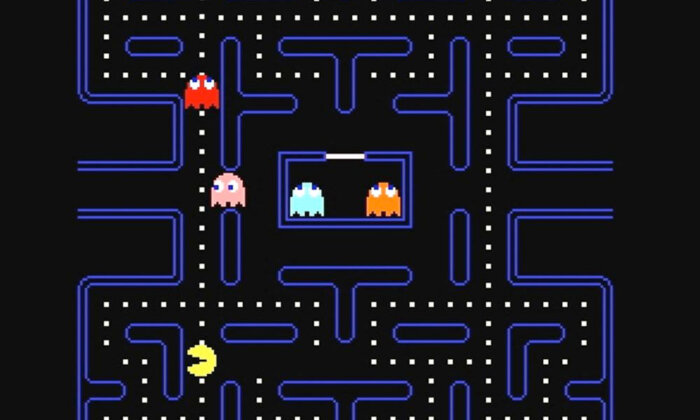
\includegraphics[scale=0.6]{pacman}
	\centering
	\caption{بازی \lr{pacman}}
	\cite{NoahWardrip}
	\label{fig2}
\end{figure} 
\section{طرح مسئله}
زیمن بازی از یک صفحه 9 در 18 درست شده است که موانع جوایزی درزمین بازی قرار گرفته شده اند . در این بازی باید با استفاده از الگوریتم 
\lr{min-max}
باید عامل هوشمند تصمیم بگیرد تا 
\lr{Pacman}
را در کدام جهت هدایت نماید . محیط بازی به صورت پویا ست و همین طور حرکت روح ها به صورت تصادفی می باشد . عامل هوشمند فرض را بر این می گذارد که در هر گام حریف یعنی روح ها بهینه ترین کار برای خودشان را انجام می دهند . در هر گام عامل با توجه به ارزش گذاری فضای حالات تصمیم می گیرد که در کدام جهت حرکت نماید . همین طور به علت این که نمی تون تا هر عمق دلخواهی در درخت حالات جست و جو نمود بایستی تابع ارزیابی طرح نمود تا بتوان با استفاده از آن خوب بودن یک حالت را بررسی نمود .
\section{کلاس ها و متد های  مورد نیاز}
در این بخش به کلاس های پیاده سازی شده می پردازیم . برای تمامی کلاس ها متد کپی برای کپی کرد هر شیء پیاده شه است .
\subsection{\lr{board}}
این کلاس کل بازی را تشکیل می دهد وشامل موانع ، جوایز ، تابع ارزیابی ، پک من و روح ها می باشد . متد هایی که برای این کلاس استفاده شده است شامل متد ارزیابی حالت فعلی 
(\lr{utility})
افزودن روح یا پک من 
( \lr{add pg} )
حرکت دادن موجودات
(\lr{move-request})
نقشه محیط
(\lr{Map})
تشخیص حالت پایانی
(\lr{is-leaf})
یک گام حرکت همه ی موجودات
(\lr{step})
 می باشند .

\subsection{\lr{PG}}
این کلاس در حقیقت یک موجود متحرک را که می تواند روح یا خود پک من باشد رامشخص می نماید و کلاس های پک من و روح از آن ارث بری می نمایند . اصلی ترین متد این کلاس 
\lr{move}
می باشد تا موجود بتواند با آن به شیء زمین بازی 
\lr{board}
 درخواست حرکت بدهد تا در صورت نبود مانع حرکت کند . 
\subsection{\lr{Pacman}}
اصلی ترین متد ها : تصمیم گیری برای این که به کدام جهت حرکت کند 
 (\lr{decsision})

جست و جوی ماکزیمم و مینیمم برای الگوریتم \lr{min-max}
 (\lr{Min-search , Max-search})

\subsection{\lr{ghost}}
کلاس روح با متد 
\lr{go}
یک جهت تصادفی انتخاب می نماید و با 
\lr{move}
در جهت آن حرکت می کند .
\section{الگوریتم هرس $\alpha$ - $\beta$}
بخش امتیازی پروژه پیاده سازی بهبودی برای سرعت الگوریتم بود که سعی شد پیاده شود .
\section{تابع ارزیابی و عمق جست و جو}
ای تابع در حالت کلی به صورت جمع وزن داری از موارد مطلوب می باشد . برای ارزیابی یک حالت امتیاز بدست آورده شده توسط پک من را محاسبه می کنیم .
\section{عملکرد الگوریتم}
بازی را تا تعداد مشخصی گام اجرا کردم و نتایج به شرح زیر می باشند :
\section{لینک گیت هاب کد}
با مراجعه به 
\url{https://github.com/mahdialipoo/AI_AUT_3}
می توانید کد مربوط به پیاده سازی این بازی را مشاهده نمایید .
